\question
Avi is coaching a robot basketball team. In order to control the team, he sends input instructions to a lead robot, which communicates the message to its team members with a delay. However, he is experiencing technical difficulties with a few of his players. They appear to be freezing up at times, resulting in bad passes, double dribbles, and all around mayhem on the court. Avi suspects it is due to synchronization problems with his robots, leading to undefined behavior.

He models each robot as a register and gives you the following schematic with a sample instruction.

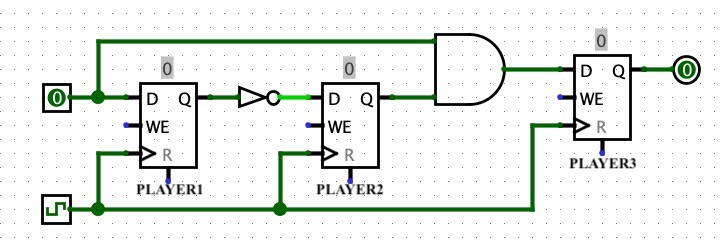
\includegraphics[width=\textwidth]{sds/bball_model}

The clock period is 16ps. Each register has a clk-to-Q delay of 4ps, a hold time of 4ps, and a setup time of 8ps. The NOT gate has a 1ps delay, and the AND gate has a 2ps delay. Help Avi find out where the output of each register is undefined!
Note that the waveforms represent the values at the OUTPUT of each register.


\begin{figure}\nopagebreak
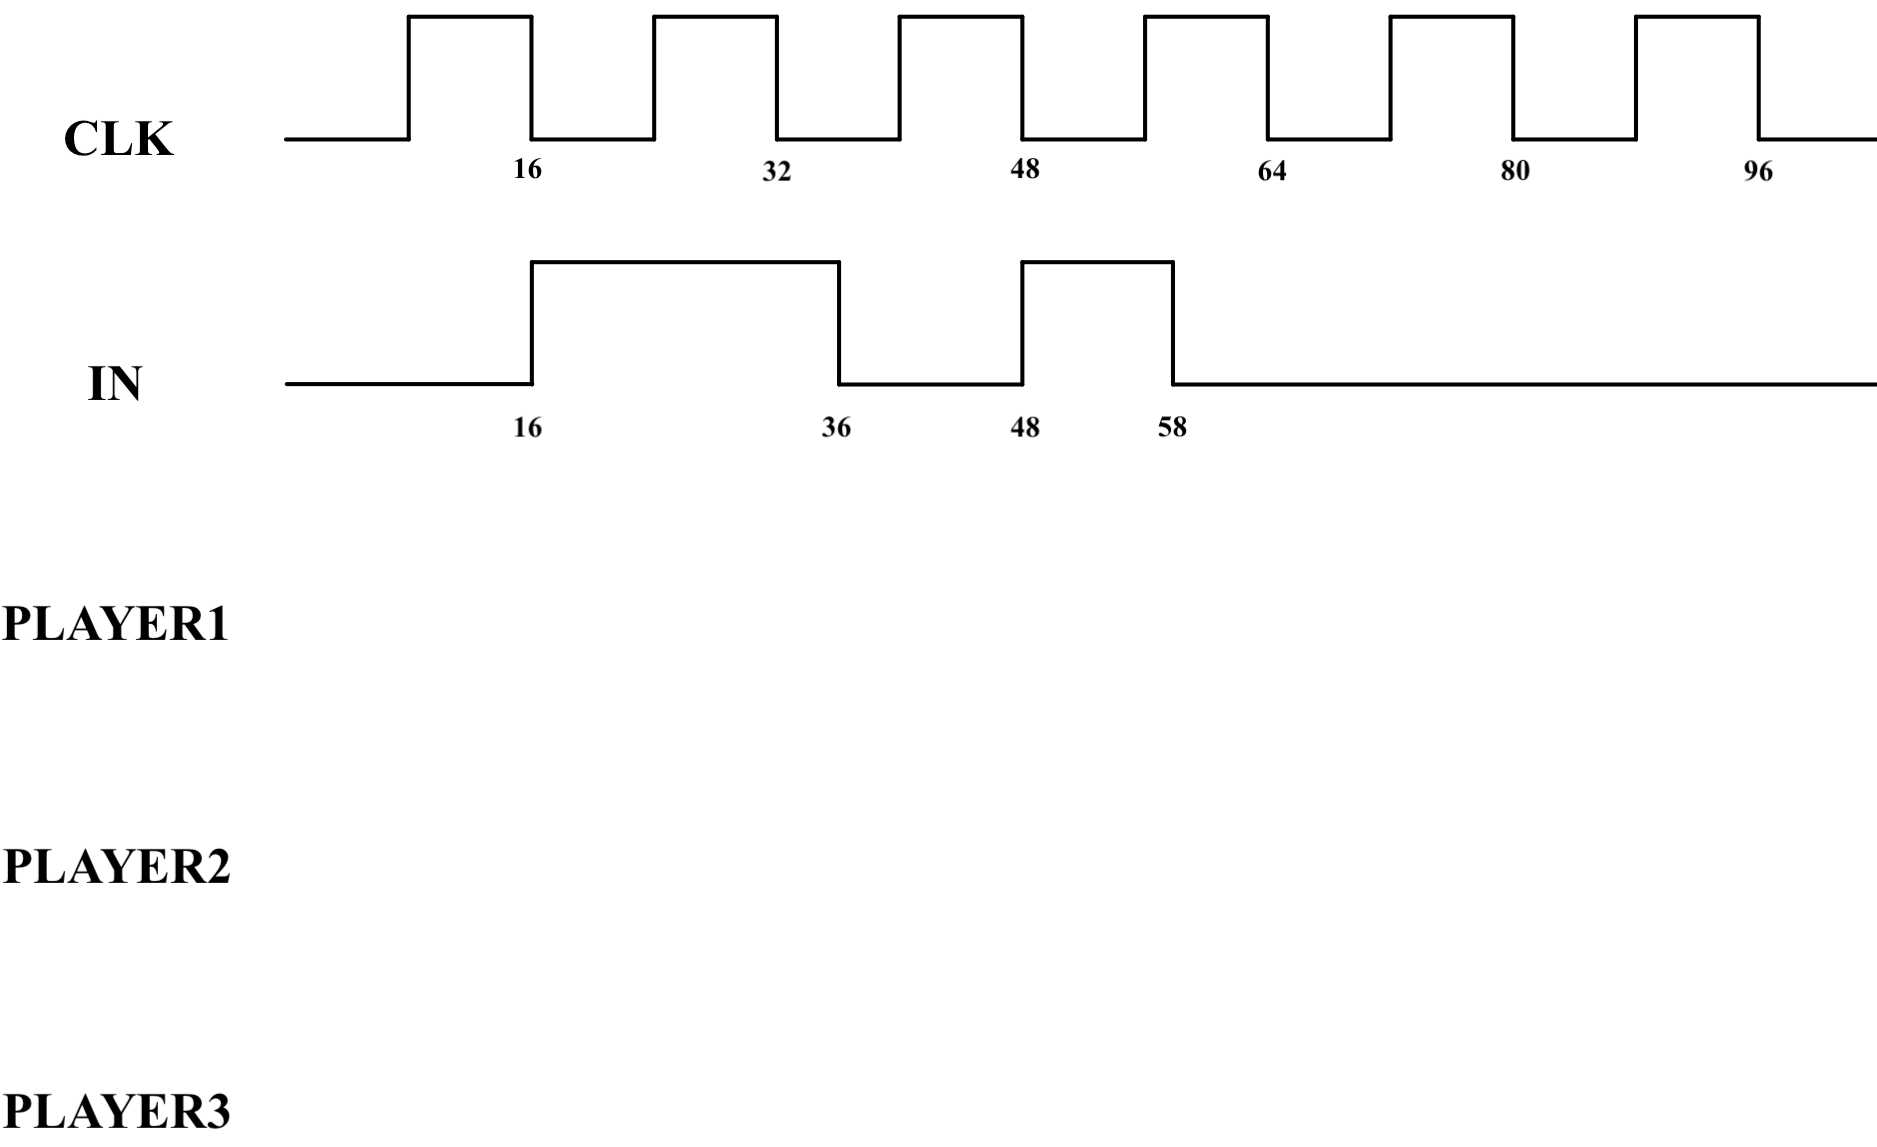
\includegraphics[width=\textwidth]{sds/bball_clock_input}\nopagebreak
\end{figure}
\nopagebreak
\begin{solution}
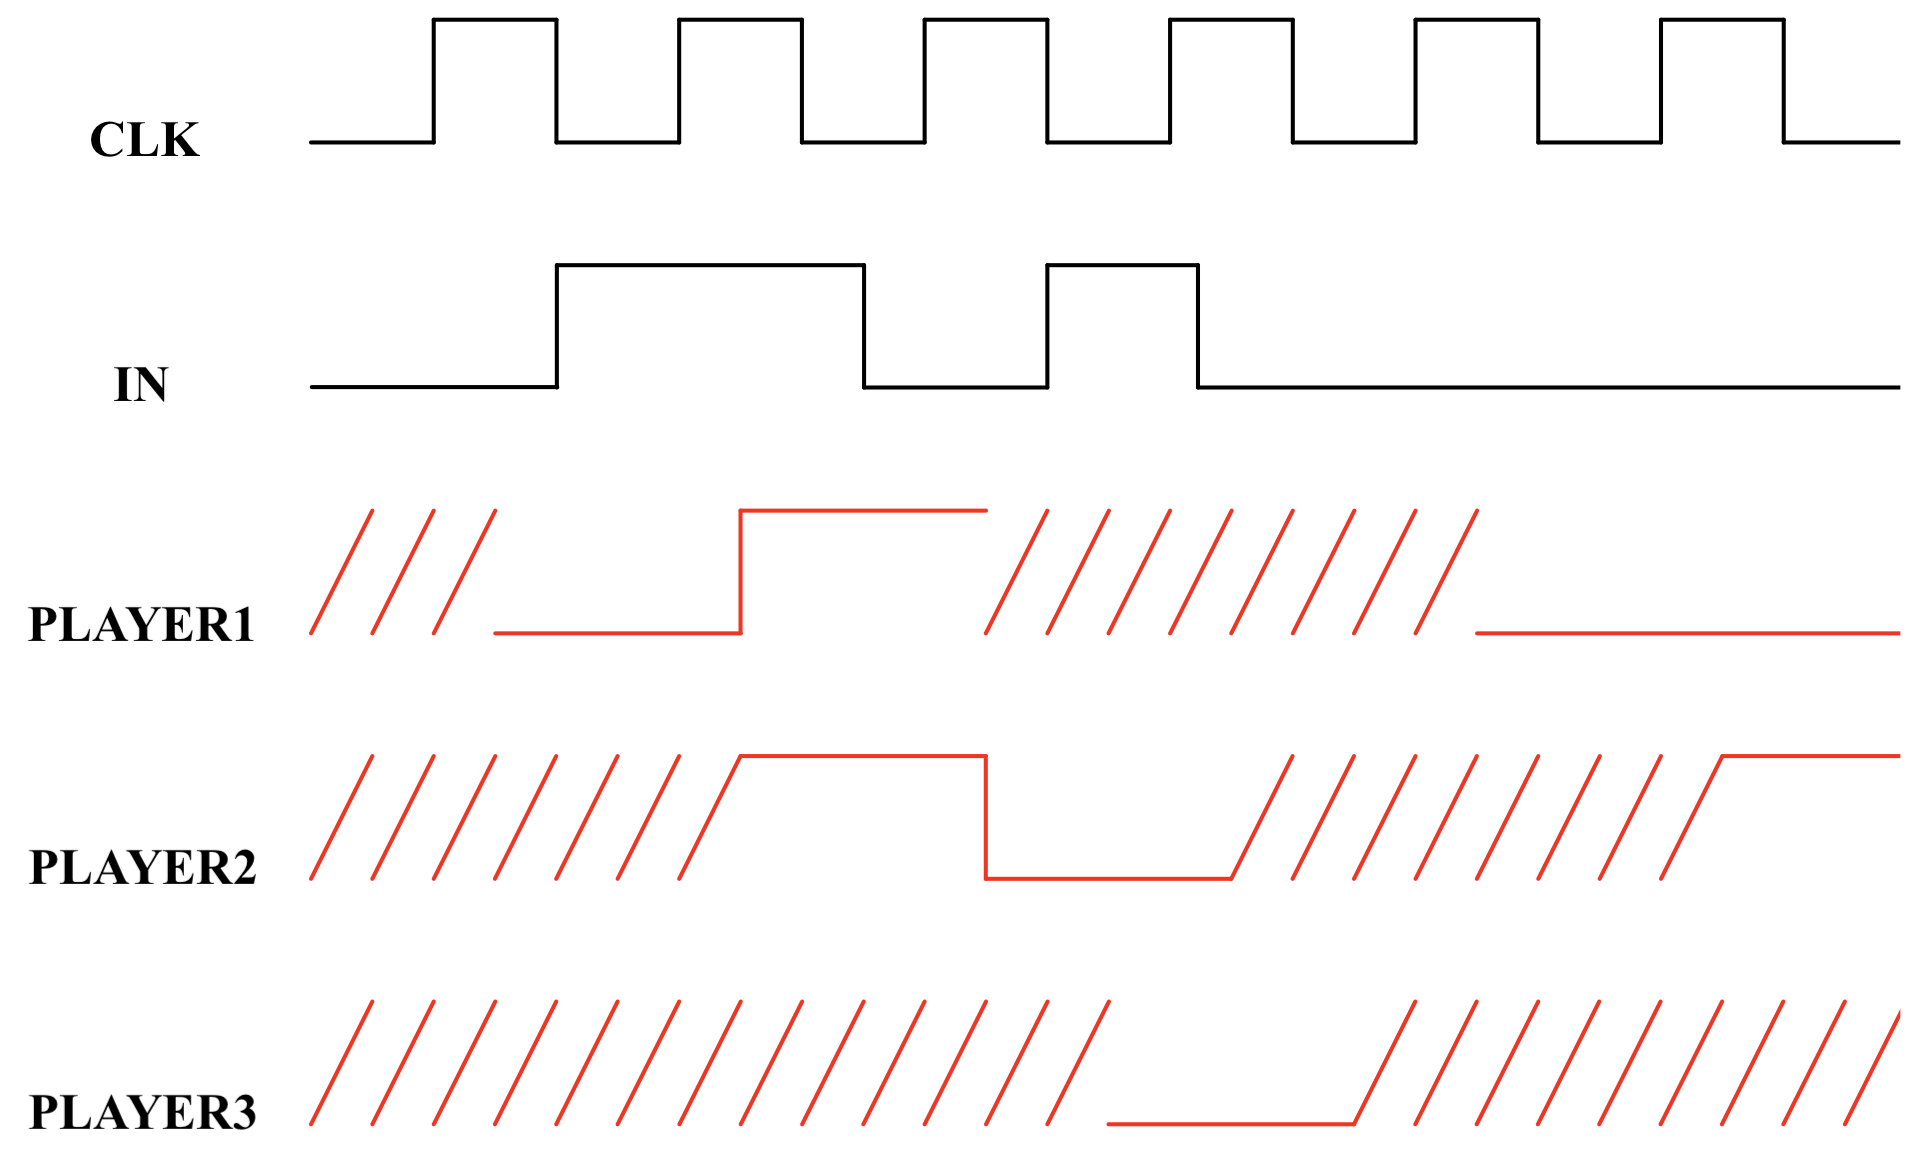
\includegraphics[width=\textwidth]{sds/bball_clock_input_sol}
\end{solution}

